\documentclass[tikz,border=7pt]{standalone}
\usetikzlibrary{arrows}
\usetikzlibrary{arrows.meta}
\usetikzlibrary{calc} 
\tikzset{>=latex}

\begin{document}
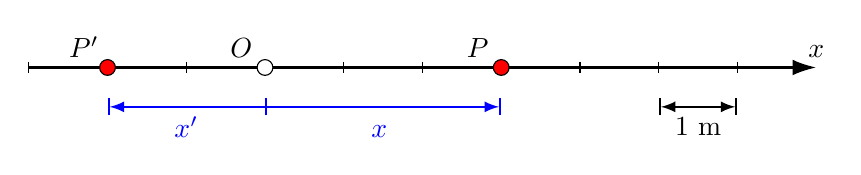
\begin{tikzpicture}[]

    \draw[-{Latex[length=3mm,width=2mm]}, thick, black] 
    (0,0) -- (10,0) node[left, above] {$x$};
    
    \foreach \x in {0,1,...,9}
    \draw (\x, 2pt) -- (\x, -2pt); % Ticks at 0.5 intervals

    
    \filldraw[fill=white] (3,0) circle [radius=1mm] node[left, above,xshift=-3mm] {$O$};

    \filldraw[draw=black,fill=red] (6,0) circle [radius=1mm] node[left, above,xshift=-3mm] {$P$};

    \filldraw[draw=black,fill=red] (1,0) circle [radius=1mm] node[left, above,xshift=-3mm] {$P^\prime$};

    \draw[|<->|, thick] (8,-0.5) -- (9,-0.5) node[midway,below] {1 m};

    \draw[blue,|->|, thick] (3,-0.5) -- (6,-0.5) node[midway,below] {$x^{\phantom{\prime}}$};

    \draw[blue,|<-, thick] (1,-0.5) -- (3,-0.5) node[midway,below] {$x^\prime$};

   
\end{tikzpicture}

\end{document}
